\documentclass{article}
\usepackage{tikz}
\usetikzlibrary{arrows.meta}
\begin{document}
	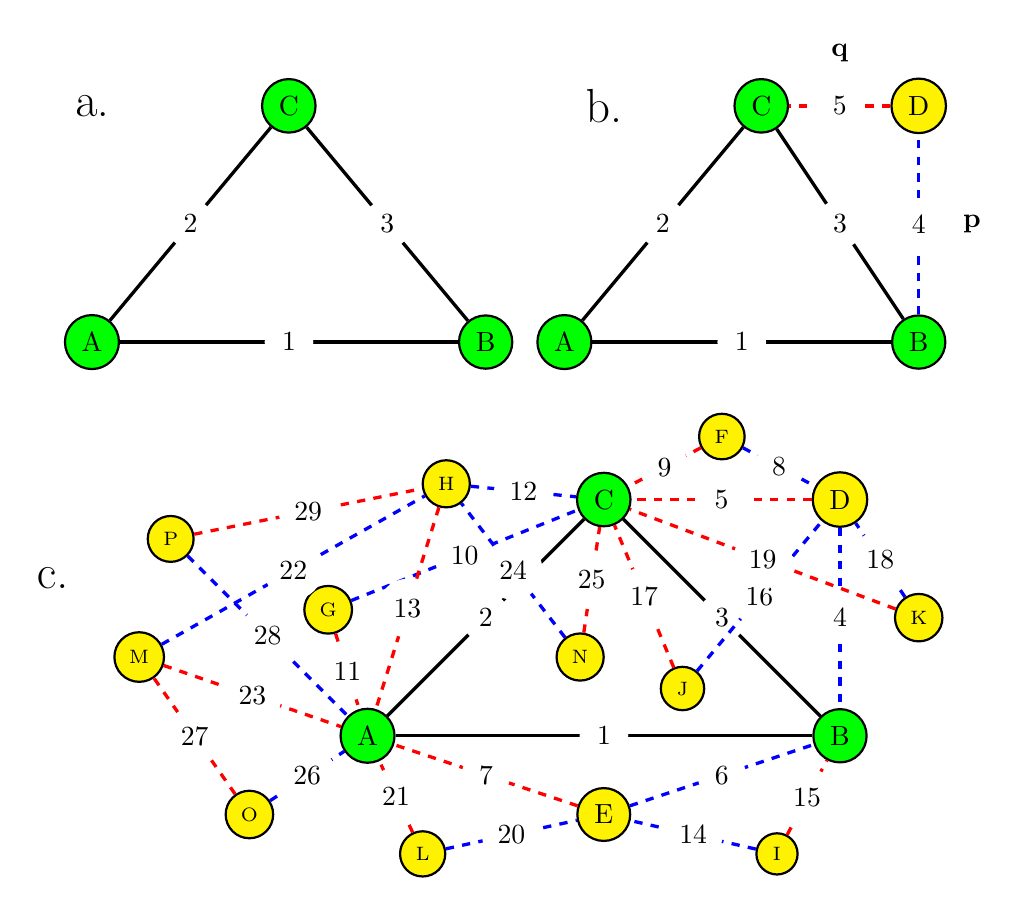
\begin{tikzpicture}
		
		
		%-----INITIAL STEP OF NETWORK FORMATION --------------------------
		
		%--------------------NODES---------------------------
				\begin{scope}[every node/.style={circle,thick,draw}]
			\node [ fill=green,text=black](A) at (-6.5,5) {A};
            \node [ fill=green,text=black] (B) at (-1.5,5) {B};
            \node[ fill=green,text=black] (C) at (-4,8) {C};
		\end{scope}
		
		%--------------------CONNECTION---------------------------
		\begin{scope}[>={Stealth[black]},
			every node/.style={fill=white,circle},
			every edge/.style={draw=black,very thick}]
			\path [-] (A) edge node {$1$} (B);
			\path [-] (A) edge node {$2$} (C);
			\path [-] (B) edge node {$3$} (C);
		\end{scope}
		
		%% LABEL INITIAL STEP OF NETWORK FORMATION as a above node A 	
		\node (a) at (-6.5,8) {\LARGE a.};
		
		
			%-----FIRST STEP OF NETWORK FORMATION --------------------------
					%--------------------NODES---------------------------
					\begin{scope}[every node/.style={circle,thick,draw}]
				\node [ fill=green,text=black](A) at (-0.5,5) {A};
                \node [ fill=green,text=black] (B) at (4,5) {B};
                \node[ fill=green,text=black] (C) at (2,8) {C};
                \node [ fill=yellow,text=black](D) at (4,8) {D};
			\end{scope}
			
			%--------------------CONNECTION---------------------------
			\begin{scope}[>={Stealth[black]},
				every node/.style={fill=white,circle},
				every edge/.style={draw=black,very thick}]
				\path [-] (A) edge node {$1$} (B);
				\path [-] (A) edge node {$2$} (C);
				\path [-] (B) edge node {$3$} (C);
			\end{scope}
			
			%--------------------CONNECT NODE D---------------------------
			\begin{scope}[>={Stealth[black]},
				every node/.style={fill=white,circle},
				every edge/.style={draw=blue,very thick}]
				\path [-,dashed] (B) edge node [label=right:\( \mathbf{p} \)] {$4$} (D);
			\end{scope}
			\begin{scope}[>={Stealth[black]},
				every node/.style={fill=white,circle},
				every edge/.style={draw=red,very thick}]
				\path [-,dashed, very thick] (D) edge node [label=above:\( \mathbf{q} \)] {$5$} (C);
			\end{scope}
			
			
					%% LABEL FIRST STEP OF NETWORK FORMATION as b above node A 	
			\node (b) at (0,8) {\LARGE b.};
			
			
			
			
			
			
%--------------------SECOND STEP OF NETWORK FORMATION---------------------------	
		
		%--------------------NODES---------------------------	
		\begin{scope}[every node/.style={circle,thick,draw}]
			\node [ fill=green,text=black](A) at (-3,0) {A};
			\node [ fill=green,text=black] (B) at (3,0) {B};
			\node[ fill=green,text=black] (C) at (0,3) {C};
			\node [ fill=yellow,text=black](D) at (3,3) {D};
			\node[fill=yellow,text=black] (E) at (0, -1.0) [] {E};
				\node[fill=yellow,text=black] (F) at (1.5,3.8) [] {\scriptsize F}; % (1.5, 4)
			    \node[fill=yellow,text=black] (G) at (-3.5, 1.6) [] {\scriptsize G}; % (-3.5, 4)
				\node[fill=yellow,text=black] (H) at (-2, 3.2) [] {\scriptsize H}; % (-1.5, 3)
			    \node[fill=yellow,text=black] (I) at (2.2, -1.5) [] {\scriptsize I};
			     \node[fill=yellow,text=black] (J) at (1, 0.6) [] {\scriptsize J}; % (5, -0.6)
			     \node[fill=yellow,text=black] (K) at (4, 1.5) [] {\scriptsize K};
				 \node[fill=yellow,text=black] (L) at (-2.3, -1.5) [] {\scriptsize L};
				 \node[fill=yellow,text=black] (M) at (-5.9, 1) [] {\scriptsize M};
%				 \node[fill=yellow,text=black] (N) at (-6, -2) [] {\scriptsize N};
                  \node[fill=yellow,text=black] (N) at (-0.3, 1) [] {\scriptsize N};
				  \node[fill=yellow,text=black] (O) at (-4.5, -1) [] {\scriptsize O};
				  \node[fill=yellow,text=black] (P) at (-5.5, 2.5) [] {\scriptsize P};
		\end{scope}
		
		%-------------CONNECTIONS----------------------------------
		
		% initial connections with solid line
		\begin{scope}[>={Stealth[black]},
			every node/.style={fill=white,circle},
			every edge/.style={draw=black,very thick}]
			\path [-] (A) edge node {$1$} (B);
			\path [-] (A) edge node {$2$} (C);
			\path [-] (B) edge node {$3$} (C);
		\end{scope}
		
		% New connections with dashed lines
		
			% CONNECTING NODE D	
		\begin{scope}[>={Stealth[black]},
			every node/.style={fill=white,circle},
			every edge/.style={draw=blue,very thick}]
			\path [-,dashed] (D) edge node [] {$4$} (B);
		\end{scope}
	
		\begin{scope}[>={Stealth[black]},
			every node/.style={fill=white,circle},
			every edge/.style={draw=red,very thick}]
			\path [-,dashed, very thick] (D) edge node [] {$5$} (C);
		\end{scope}
	
	
			% CONNECTING NODE E	
			
				
			\begin{scope}[>={Stealth[black]},
				every node/.style={fill=white,circle},
				every edge/.style={draw=blue,very thick}]
				\path [-,dashed, very thick] (E) edge node [] {$6$} (B);
			\end{scope}
		\begin{scope}[>={Stealth[black]},
			every node/.style={fill=white,circle},
			every edge/.style={draw=red,very thick}]
			\path [-,dashed, very thick] (E) edge node [] {$7$} (A);
		\end{scope}

		
			% CONNECTING NODE F
					\begin{scope}[>={Stealth[black]},
			every node/.style={fill=white,circle},
			every edge/.style={draw=blue,very thick}]
			\path [-,dashed, very thick] (F) edge node [] {$8$} (D);
		\end{scope}
		
		\begin{scope}[>={Stealth[black]},
			every node/.style={fill=white,circle},
			every edge/.style={draw=red,very thick}]
			\path [-,dashed, very thick] (F) edge node [] {$9$} (C);
		\end{scope}
	

			% CONNECTING NODE G
			\begin{scope}[>={Stealth[black]},
				every node/.style={fill=white,circle},
				every edge/.style={draw=blue,very thick}]
				\path [-,dashed, very thick] (G) edge node [] {$10$} (C);
			\end{scope}
				\begin{scope}[>={Stealth[black]},
			every node/.style={fill=white,circle},
			every edge/.style={draw=red,very thick}]
			\path [-,dashed, very thick] (G) edge node [] {$11$} (A);
		\end{scope}
		


		% CONNECTING NODE H	
		
			\begin{scope}[>={Stealth[black]},
			every node/.style={fill=white,circle},
			every edge/.style={draw=blue,very thick}]
			\path [-,dashed, very thick] (H) edge node [] {$12$} (C);
		\end{scope}
	
	\begin{scope}[>={Stealth[black]},
		every node/.style={fill=white,circle},
		every edge/.style={draw=red,very thick}]
		\path [-,dashed, very thick] (H) edge node [] {$13$} (A);
	\end{scope}
	

	
	
			% CONNECTING NODE I	
			
				\begin{scope}[>={Stealth[black]},
				every node/.style={fill=white,circle},
				every edge/.style={draw=blue,very thick}]
				\path [-,dashed, very thick] (I) edge node [] {$14$} (E);
			\end{scope}
			
	\begin{scope}[>={Stealth[black]},
		every node/.style={fill=white,circle},
		every edge/.style={draw=red,very thick}]
		\path [-,dashed, very thick] (I) edge node [] {$15$} (B);
	\end{scope}
	
				% CONNECTING NODE J	
	\begin{scope}[>={Stealth[black]},
		every node/.style={fill=white,circle},
		every edge/.style={draw=blue,very thick}]
		\path [-,dashed, very thick] (J) edge node [] {$16$} (D);
	\end{scope}
	
	\begin{scope}[>={Stealth[black]},
		every node/.style={fill=white,circle},
		every edge/.style={draw=red,very thick}]
		\path [-,dashed, very thick] (J) edge node [] {$17$} (C);
	\end{scope}
	
	
					% CONNECTING NODE K	
	\begin{scope}[>={Stealth[black]},
		every node/.style={fill=white,circle},
		every edge/.style={draw=blue,very thick}]
		\path [-,dashed, very thick] (K) edge node [] {$18$} (D);
	\end{scope}
	
	\begin{scope}[>={Stealth[black]},
		every node/.style={fill=white,circle},
		every edge/.style={draw=red,very thick}]
		\path [-,dashed, very thick] (K) edge node [] {$19$} (C);
	\end{scope}
	
	
						% CONNECTING NODE L	
			\begin{scope}[>={Stealth[black]},
			every node/.style={fill=white,circle},
			every edge/.style={draw=blue,very thick}]
			\path [-,dashed, very thick] (L) edge node [] {$20$} (E);
		\end{scope}
						
	\begin{scope}[>={Stealth[black]},
		every node/.style={fill=white,circle},
		every edge/.style={draw=red,very thick}]
		\path [-,dashed, very thick] (L) edge node [] {$21$} (A);
	\end{scope}
	

	
	
						% CONNECTING NODE M	
	\begin{scope}[>={Stealth[black]},
		every node/.style={fill=white,circle},
		every edge/.style={draw=blue,very thick}]
		\path [-,dashed, very thick] (M) edge node [] {$22$} (H);
	\end{scope}
	
	\begin{scope}[>={Stealth[black]},
		every node/.style={fill=white,circle},
		every edge/.style={draw=red,very thick}]
		\path [-,dashed, very thick] (M) edge node [] {$23$} (A);
	\end{scope}
	
	
						% CONNECTING NODE N	
	\begin{scope}[>={Stealth[black]},
	every node/.style={fill=white,circle},
	every edge/.style={draw=blue,very thick}]
	\path [-,dashed, very thick] (N) edge node [] {$24$} (H);
\end{scope}

\begin{scope}[>={Stealth[black]},
	every node/.style={fill=white,circle},
	every edge/.style={draw=red,very thick}]
	\path [-,dashed, very thick] (N) edge node [] {$25$} (C);
\end{scope}


						% CONNECTING NODE O	
\begin{scope}[>={Stealth[black]},
	every node/.style={fill=white,circle},
	every edge/.style={draw=blue,very thick}]
	\path [-,dashed, very thick] (O) edge node [] {$26$} (A);
\end{scope}

\begin{scope}[>={Stealth[black]},
	every node/.style={fill=white,circle},
	every edge/.style={draw=red,very thick}]
	\path [-,dashed, very thick] (O) edge node [] {$27$} (M);
\end{scope}


						% CONNECTING NODE P	
\begin{scope}[>={Stealth[black]},
	every node/.style={fill=white,circle},
	every edge/.style={draw=blue,very thick}]
	\path [-,dashed, very thick] (P) edge node [] {$28$} (A);
\end{scope}

\begin{scope}[>={Stealth[black]},
	every node/.style={fill=white,circle},
	every edge/.style={draw=red,very thick}]
	\path [-,dashed, very thick] (P) edge node [] {$29$} (H);
\end{scope}



%% LABEL SECOND STEP OF NETWORK FORMATION as c above node M 	
\node (c) at (-7,2) {\LARGE c.};

	\end{tikzpicture}
\end{document}